\documentclass[11pt,a4paper]{article}

% ===== Packages =====
\usepackage[utf8]{inputenc}
\usepackage[T1]{fontenc}
\usepackage{amsmath,amssymb,amsthm,mathtools}
\usepackage{geometry}
\geometry{margin=1in}
\usepackage{graphicx}
\graphicspath{{../figures/}}
\usepackage{hyperref}
\usepackage{cleveref}
\usepackage{natbib}
\usepackage{booktabs}
\usepackage{algorithm}
\usepackage{algorithmic}
\usepackage{tikz}
\usepackage{subcaption}
\usepackage{xcolor}
\usepackage{enumitem}
\usepackage{microtype}
\usepackage{tabularx}
\usepackage[section]{placeins}

% ===== Theorem environments =====
\newtheorem{claim}{Claim}[section]
\newtheorem{conjecture}[claim]{Conjecture}
\theoremstyle{definition}
\newtheorem{definition}[claim]{Definition}
\newtheorem{example}[claim]{Example}
\newtheorem{remark}[claim]{Remark}
\newtheorem{assumption}[claim]{Assumption}

% ===== Notation =====
\newcommand{\R}{\mathbb{R}}
\newcommand{\E}{\mathbb{E}}
\newcommand{\KL}{\mathrm{KL}}
\newcommand{\VFE}{\mathcal{F}}
\newcommand{\EFE}{\mathcal{G}}
\newcommand{\cA}{\mathcal{A}}
\newcommand{\cS}{\mathcal{S}}
\newcommand{\cO}{\mathcal{O}}
\newcommand{\cM}{\mathcal{M}}
\newcommand{\cP}{\mathcal{P}}
\newcommand{\cW}{\mathcal{W}}
\newcommand{\cC}{\mathcal{C}}
\newcommand{\cF}{\mathcal{F}}  % sigma-algebra in probability spaces
\newcommand{\cB}{\mathcal{B}}
\newcommand{\cT}{\mathcal{T}}
\newcommand{\Wass}{W_2}
\newcommand{\FI}{\mathcal{I}}
\newcommand{\mani}{\mathcal{M}}
\newcommand{\dkl}{D_{\mathrm{KL}}}
\newcommand{\supp}{\mathrm{supp}}

\title{A Framework for Modeling and Steering Agent Belief Structures \\ via Active Inference and Geodesic Paths}

\author{
  Mahault Albarracin\textsuperscript{1,2,3} \and
  Dalton Sakthivadivel\textsuperscript{4} \and
  Nicol\'{a}s Hinrichs\textsuperscript{5} \and
  David Hyland\textsuperscript{6} \and
  Gabriel Axel Montes\textsuperscript{7} \and
  Ben Goertzel\textsuperscript{8}
}

\date{
  \textsuperscript{1}LANCI, Universit\'{e} du Qu\'{e}bec \`{a} Montr\'{e}al \\
  \textsuperscript{2}School of Computing and Digital Technologies, Sheffield Hallam University \\
  \textsuperscript{3}ISS \& IREF, Universit\'{e} du Qu\'{e}bec \`{a} Montr\'{e}al \\
  \textsuperscript{4}CUNY Graduate Center \\
  \textsuperscript{5}Max Planck Institute for Human Cognitive and Brain Sciences \\
  \textsuperscript{6}Department of Computer Science, University of Oxford \\
  \textsuperscript{7}University of Newcastle, Australia \\
  \textsuperscript{8}ASI Alliance / SingularityNET Foundation
}

\begin{document}

\maketitle

\begin{abstract}
Current approaches to AI alignment often compare outputs or belief distributions while omitting the dynamics that produce them. We propose a five-phase geometric framework for comparing belief-generating systems through attractor topology, dynamical operators, transport geometry, hierarchical co-steering, and explicit normative constraints. A deterministic rerun of the current synthetic belief-network pipeline separates deliberately constructed rigid and flexible regimes (mean-persistence ratio $3.79\times$) and reproduces sensitivity to a prior-precision perturbation (direction change $0.5517$). Earlier exploratory cryptocurrency, EEG, and Reddit analyses suggest possible real-data applications, but their datasets and machine-readable result ledgers are absent from the present checkout and their numerical claims were not reproduced in the current audit. The framework therefore supplies a mathematical and experimental research programme, not yet a validated measure of real-world or moral alignment.
\end{abstract}

\noindent\textbf{Keywords.} Active inference, information geometry, alignment, belief dynamics, random dynamical systems, persistent homology, optimal transport, Schr\"{o}dinger bridges


\section{Introduction}
\label{sec:introduction}

The alignment problem, ensuring that artificial agents act in accordance with human values and intentions, has become a central concern of AI safety research \citep{gabriel2020artificial, russell2019human}. Current approaches predominantly operate at the level of agent \emph{outputs}: reinforcement learning from human feedback (RLHF) shapes policy behavior through preference comparisons \citep{christiano2017deep, ouyang2022training}, constitutional AI encodes principles as textual constraints \citep{bai2022constitutional}, and reward modeling learns scalar proxies for human satisfaction. When alignment is formalized mathematically, the default tool is Kullback--Leibler divergence, comparing the distribution an agent produces against a target distribution.

We argue that all such approaches share a fundamental limitation: they compare the \emph{products} of belief-generating processes rather than the processes themselves. Consider two agents whose current belief distributions are identical, say, both assign 60\% probability to proposition $p$. Standard metrics declare them equally aligned. Yet one agent may inhabit a deep, rigid attractor basin with high precision and dogmatic updating while the other occupies a shallow, flexible basin with low precision and exploratory updating. Their responses to novel evidence, social influence, and adversarial perturbation will diverge dramatically. The first agent is brittle: aligned today, catastrophically misaligned tomorrow if the attractor shifts. The second is robust: capable of tracking a changing world.

This paper develops a geometric framework that captures these distinctions. Our central thesis is:
\begin{quote}
\emph{Alignment should be understood as the distance between belief-generating dynamical systems, their attractor landscapes, geodesic flows, and curvature structure, not as the distance between the beliefs they currently produce.}
\end{quote}

We formalize this thesis through five phases. Phase~1 (\Cref{sec:phase1}) establishes the topology of beliefs by mapping generative models onto statistical manifolds and reconstructing their attractor structure via persistent homology and random dynamical systems theory. Phase~1.5 (\Cref{sec:phase1p5}) grounds these mathematical structures in psychological and cognitive interpretation, connecting basin depth to cognitive rigidity, ridges to identity barriers, and funnels to convergent narratives. Phase~2 (\Cref{sec:phase2}) quantifies misalignment as topological distance between belief-generating systems, adopting $C^*$-algebra homomorphisms on RDS attractors after evaluating and rejecting KL divergence and Gromov--Hausdorff distance. Phase~3 (\Cref{sec:phase3}) models belief path dynamics by bridging variational inference with Wasserstein gradient flows and applying a Freidlin--Wentzell large deviation principle to identify least-surprise belief geodesics. Phase~4 (\Cref{sec:phase4}) develops hierarchical co-steering through curvature mapping, empowerment constraints, and Mori--Zwanzig coarse-graining. Finally, Phase~4.5 (\Cref{sec:phase4p5}) establishes normative criteria for beneficial attractor landscapes, including epistemic adequacy, empowerment preservation, cooperative compatibility, and pluralism.

We validate the framework through three experiments combining controlled simulations with real-world data (\Cref{sec:experiments}): a synthetic belief network with cryptocurrency market validation demonstrating that RDS distances capture structural misalignment invisible to KL divergence; real EEG hyperscanning data from cooperative and competitive dyads showing that Forman--Ricci curvature dynamics predict task condition; and Reddit political communities revealing echo chambers as topologically distinct belief basins with measurably different persistence signatures.

\Cref{fig:framework_overview} illustrates the core intuition: two attractor basins on a belief landscape connected by a surprise geodesic, with the ridge between them encoding the cost of transitioning from one worldview to another.

\begin{figure}[!htbp]
  \centering
  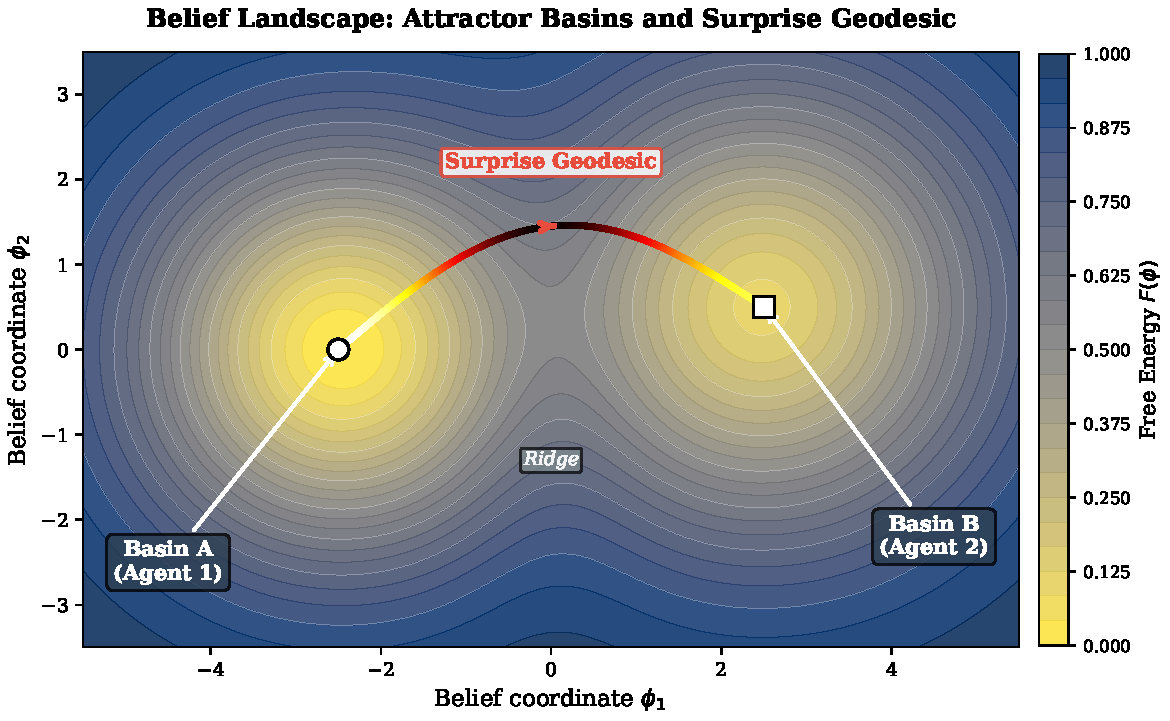
\includegraphics[width=0.85\textwidth]{fig_framework_overview.pdf}
  \caption{Schematic of the belief landscape. Two attractor basins (representing distinct worldviews or agent types) are separated by a ridge encoding the cognitive, affective, and social cost of belief change. The surprise geodesic traces the most likely transition path between basins, the trajectory that deviates least from the free energy gradient. Basin depth corresponds to belief rigidity; ridge height corresponds to the difficulty of alignment.}
  \label{fig:framework_overview}
\end{figure}

Our main contributions are fivefold. First, we provide a formal framework unifying active inference, information geometry, random dynamical systems, and optimal transport into a geometric theory of alignment. Second, we introduce the RDS homomorphism metric for misalignment, which compares belief-generating dynamical systems rather than belief distributions. Third, we establish the variational--Wasserstein bridge, connecting parameter-space gradient descent on variational free energy with Wasserstein geodesics on belief space. Fourth, we derive a Freidlin--Wentzell extension identifying least-surprise belief paths as the most likely trajectories of stochastic belief updating. Fifth, we provide empirical validation through controlled synthetic experiments spanning belief networks, neural oscillators, and simulated online communities, demonstrating that topological structure predicts alignment dynamics where distributional metrics fail.


\section{Background and Related Work}
\label{sec:background}

The framework draws on five bodies of mathematics and situates itself against existing alignment approaches. We review each in turn, emphasizing the connections that the subsequent phases exploit.

\subsection{Active Inference and Free Energy}
\label{sec:bg_aif}

Active inference casts perception, learning, and action as approximate Bayesian inference under a single imperative: minimize variational free energy \citep{friston2010free, parr2022active}. An agent maintains a generative model $p(o, s \mid \theta)$ over observations $o \in \cO$ and hidden states $s \in \cS$, parameterized by $\theta$. Given observations, the agent updates an approximate posterior $q(s; \phi)$ by minimizing the variational free energy (VFE):
\begin{equation}
  \VFE[q, o] = \dkl\bigl[q(s; \phi) \,\|\, p(s \mid o, \theta)\bigr] - \ln p(o \mid \theta)
  \label{eq:vfe}
\end{equation}
which bounds the negative log-evidence $-\ln p(o \mid \theta)$ from above. For action selection, the agent evaluates policies $\pi$ by their expected free energy (EFE):
\begin{equation}
  \EFE(\pi) = \sum_{\tau} \E_{q(o_\tau, s_\tau \mid \pi)}\bigl[\ln q(s_\tau \mid \pi) - \ln p(o_\tau \mid C) - \ln p(s_\tau \mid o_\tau)\bigr]
  \label{eq:efe}
\end{equation}
where $C$ encodes preferred observations and $p(s_\tau \mid o_\tau)$ is the generative model's posterior. Under this formulation, the expected posterior divergence contributes epistemic value, while $-\ln p(o_\tau \mid C)$ is expected negative log preference, or pragmatic cost. EFE is also commonly expressed in risk--ambiguity form, but the equality among decompositions depends on the root EFE definition, factorization, preference representation, and approximation assumptions; these forms should not be interchanged without stating those conditions \citep{parr2022active,millidge2021whence}. Policy selection follows a softmax $p(\pi) = \sigma\bigl(-\gamma \, \EFE(\pi)\bigr)$ with precision parameter $\gamma$ controlling sensitivity to expected policy value.

The key insight for our framework is that the generative model $p(o, s \mid \theta)$ induces a point on a statistical manifold, and the free energy gradient $\nabla_\phi \VFE$ defines a flow on this manifold. Alignment, in these terms, concerns the relationship between the manifold geometries of different agents' generative models.

\subsection{Statistical Manifolds and Information Geometry}
\label{sec:bg_ig}

A statistical manifold $(\cM, g)$ is a smooth manifold whose points are probability distributions, equipped with the Fisher--Rao metric \citep{amari2016information}:
\begin{equation}
  g_{ij}(\theta) = \E_{p(x|\theta)}\left[\frac{\partial \ln p(x|\theta)}{\partial \theta_i} \frac{\partial \ln p(x|\theta)}{\partial \theta_j}\right]
  \label{eq:fisher_rao}
\end{equation}
For exponential family distributions $p(x \mid \theta) = h(x) \exp\bigl(\theta^\top T(x) - A(\theta)\bigr)$, the Fisher matrix coincides with the Hessian of the log-partition function: $g_{ij} = \partial^2 A / \partial \theta_i \partial \theta_j$. The natural gradient \citep{amari1998natural} accounts for the Riemannian structure via $\tilde{\nabla}_\theta \VFE = g(\theta)^{-1} \nabla_\theta \VFE$, ensuring that parameter updates respect the intrinsic geometry of the distribution family.

Crucially, the statistical manifold distinguishes the \emph{parameter space} $\Theta$ from the \emph{belief space} $\cP(\cS)$, the space of distributions over hidden states. A generative model maps parameters $\theta$ to beliefs $q(s; \phi(\theta))$. Different parameterizations can induce the same belief, and the same parameter can induce different beliefs under different generative models. Our framework operates on both levels: parameter evolution in the variational dynamics of Phase~3, and belief evolution in the Wasserstein dynamics of the same phase.

\subsection{Random Dynamical Systems and Topological Data Analysis}
\label{sec:bg_rds}

A metric random dynamical system (RDS) consists of a probability space $(\Omega, \cF, \mathbb{P})$ with an ergodic measure-preserving flow $\vartheta_t: \Omega \to \Omega$ and a cocycle $\varphi: \R_{\geq 0} \times \Omega \times X \to X$ over a complete separable metric space $(X, d)$, satisfying $\varphi(0, \omega, \cdot) = \mathrm{id}_X$ and $\varphi(s+t, \omega, x) = \varphi(s, \vartheta_t \omega, \varphi(t, \omega, x))$ for all $s, t \geq 0$, $\omega \in \Omega$, $x \in X$ \citep{arnold1998random}.

\begin{definition}[Pullback attractor]
\label{def:pullback_attractor}
A family $\{A(\omega)\}_{\omega \in \Omega}$ of compact subsets of $X$ is a \emph{pullback attractor} for the RDS $\varphi$ if it is invariant ($\varphi(t, \omega, A(\omega)) = A(\vartheta_t \omega)$ for all $t \geq 0$) and pullback-attracts all bounded sets $B$: $\lim_{t \to \infty} d_H\bigl(\varphi(t, \vartheta_{-t}\omega, B), A(\omega)\bigr) = 0$, where $d_H$ denotes the Hausdorff distance \citep{crauel1994attractors}.
\end{definition}

In our framework, each agent's belief dynamics constitute an RDS on the statistical manifold, driven by stochastic observations. The pullback attractors capture the long-term invariant structures of belief formation, the ``shapes'' that persist across observation histories. Ribbon-shaped nonequilibrium steady states \citep{sakthivadivel2024ribbon} extend this picture: when steady-state distributions are supported on lower-dimensional manifolds rather than point attractors, they generate multimodal, path-dependent belief distributions whose pathwise attractors become the objects our metric compares.

Persistent homology \citep{edelsbrunner2000topological, carlsson2009topology} provides the computational bridge between observed trajectories and topological structure. Given a point cloud $X \subset \R^d$, a filtration of simplicial complexes indexed by a scale parameter $\epsilon$ yields persistence diagrams $\mathrm{Dgm}_k(X)$ that record the birth and death of $k$-dimensional homological features as $\epsilon$ varies. Persistent features with large persistence $|d_i - b_i|$ represent robust topological structure, while short-lived features typically reflect noise. The bottleneck distance $d_B(\mathrm{Dgm}_1, \mathrm{Dgm}_2) = \inf_\gamma \sup_{x} \|x - \gamma(x)\|_\infty$ provides a stable metric for comparing topological structures. For time-series data, Takens embedding \citep{takens1981detecting} reconstructs attractor topology from scalar observables via delay coordinates $\mathbf{x}_t = (x_t, x_{t-\tau}, \ldots, x_{t-(d_e-1)\tau})$, yielding topological fingerprints of the generating dynamical system even without access to its equations of motion.

\subsection{Optimal Transport and Wasserstein Geometry}
\label{sec:bg_ot}

The 2-Wasserstein distance between probability measures $\mu, \nu \in \cP_2(\R^d)$ is
\begin{equation}
  \Wass(\mu, \nu) = \left(\inf_{\pi \in \Pi(\mu, \nu)} \int \|x - y\|^2 \, d\pi(x, y)\right)^{1/2}
  \label{eq:wasserstein}
\end{equation}
where $\Pi(\mu, \nu)$ denotes the set of couplings with marginals $\mu$ and $\nu$ \citep{villani2008optimal}. The Benamou--Brenier formula \citep{benamou2000computational} recasts this as a geodesic problem: $\Wass(\mu_0, \mu_1)^2 = \inf_{(\rho_t, v_t)} \int_0^1 \int \|v_t(x)\|^2 \, d\rho_t(x) \, dt$ subject to the continuity equation $\partial_t \rho_t + \nabla \cdot (\rho_t v_t) = 0$, revealing optimal transport as geodesic motion on the Wasserstein manifold $(\cP_2, \Wass)$.

The JKO scheme \citep{jordan1998variational} provides the critical connection to free energy: the Fokker--Planck equation $\partial_t \rho = \nabla \cdot (\rho \nabla V) + \sigma \Delta \rho$ can be interpreted as Wasserstein gradient flow of the free energy functional $\cF[\rho] = \int V \, d\rho + \sigma \int \rho \ln \rho \, dx$. This equivalence is central to our variational--Wasserstein bridge in \Cref{sec:phase3}. Finally, Schr\"{o}dinger bridges \citep{leonard2013survey, chen2021stochastic} solve the entropy-regularized transport problem $Q^* = \arg\min_{Q: Q_0 = \mu, Q_T = \nu} \dkl(Q \| P)$ where $P$ is a reference process. The SB is the most likely stochastic evolution connecting two marginals, directly related to our least-surprise geodesics and developed extensively by \citet{goertzel2025judging} for multi-agent coordination.

\subsection{Existing Alignment Approaches}
\label{sec:bg_alignment}

Current alignment methods operate at distinct levels of abstraction, none of which capture generative structure. Behavioral alignment through RLHF and preference learning compares outputs to human preferences, effective for surface behavior but silent on internal dynamics \citep{christiano2017deep, ouyang2022training}. Distributional alignment via KL minimization or $f$-divergences compares output distributions, but compresses the entire attractor landscape into a single divergence value. Constitutional and rule-based alignment encodes principles as constraints, requiring explicit value articulation and remaining brittle to novel situations \citep{bai2022constitutional}. Mechanistic interpretability examines internal representations \citep{elhage2022superposition, conmy2023towards}, capturing structure but lacking a formal distance metric between agents.

The gap is clear: no existing approach compares the \emph{dynamical systems} that generate beliefs. A rigid agent and a flexible agent with identical current outputs are indistinguishable to all of the above. Our framework fills this gap by operating on the attractor landscape itself.


\section{The Geometric Framework}
\label{sec:framework}

\subsection{Phase 1: Formalizing the Topology of Beliefs}
\label{sec:phase1}

We begin by establishing the mathematical objects whose topology we wish to compare. An agent's generative model $p(o, s \mid \theta)$ defines a point $\theta$ on a statistical manifold $\cM$. As the agent receives observations and updates its beliefs, $\theta$ traces a trajectory on $\cM$. The topology of this trajectory, its attractor structure, dimensionality, and connectivity, encodes the agent's epistemic character.

\begin{definition}[Belief trajectory]
\label{def:belief_trajectory}
Given an agent with generative model $p(o, s \mid \theta)$ and approximate posterior $q(s; \phi_t)$, the \emph{belief trajectory} is the time-indexed curve $\phi: [0, T] \to \cM$ defined by the sequence of variational parameters obtained through free energy minimization:
\begin{equation}
  \phi_{t+1} = \phi_t - \eta \, g(\phi_t)^{-1} \nabla_\phi \VFE[q(\cdot; \phi_t), o_t]
  \label{eq:belief_trajectory}
\end{equation}
where $g$ is the Fisher--Rao metric and $o_t$ are observations sampled from the environment.
\end{definition}

A critical distinction separates two levels of attractor. A \emph{state-space attractor} is a subset $A \subset \cS$ on which the probability mass $p(s \mid o_{1:T})$ concentrates as $T \to \infty$, describing \emph{what} the agent believes about the world. A \emph{belief-space attractor} is a subset $\hat{A} \subset \cM$ to which the belief trajectory $\phi_t$ converges, describing \emph{how} the agent forms and maintains beliefs. Our framework operates primarily at the belief-space level, but structure cannot replace content: topologically equivalent attractors can encode opposed beliefs or values. Epistemic and normative comparison must therefore combine the dynamics of $\hat{A}$ with semantic labels, transition direction, control costs, and effects on other agents.

Given observed belief trajectories $\{\phi_t\}_{t=1}^T$, we reconstruct the attractor topology through a four-stage pipeline. First, for scalar or low-dimensional observables, we construct Takens delay embeddings with delay $\tau$ chosen by mutual information minimization and dimension $d_e$ by false nearest neighbors \citep{takens1981detecting, kennel1992determining}. Second, we compute the Vietoris--Rips filtration on the embedded point cloud and extract persistence diagrams $\mathrm{Dgm}_k$ for $k = 0, 1, 2$: connected components ($k=0$) identify distinct attractor basins, loops ($k=1$) identify limit cycles or quasi-periodic orbits, and voids ($k=2$) reveal higher-order topological structure. Third, for smooth belief landscapes, we compute the gradient flow of VFE on $\cM$ and identify critical points through Morse-theoretic decomposition: minima correspond to attractors, saddles to basin boundaries, and maxima to repellers. Fourth, for stochastic trajectories, we apply the RDS framework (\Cref{def:pullback_attractor}) to capture the invariant structure that persists across different realizations of the observation noise.

\begin{claim}[Topological stability]
\label{claim:topo_stability}
Let $\{\phi_t^{(n)}\}$ be belief trajectories of agent $n$ and let $\hat{A}^{(n)}$ be the reconstructed attractor. Under mild regularity conditions (the generative model has bounded Fisher information and observations are sub-Gaussian), the persistence diagram $\mathrm{Dgm}_k(\hat{A}^{(n)})$ is stable: for any $\delta$-perturbation of the observations,
\begin{equation}
  d_B\bigl(\mathrm{Dgm}_k(\hat{A}^{(n)}), \mathrm{Dgm}_k(\hat{A}^{(n)}_\delta)\bigr) \leq C \delta
  \label{eq:topo_stability}
\end{equation}
for a constant $C$ depending on the Fisher information bound.
\end{claim}

The argument follows from the stability theorem for persistent homology \citep{cohen2007stability} combined with the regularity of the belief trajectory map $o_{1:T} \mapsto \{\phi_t\}$. Bounded Fisher information ensures the natural gradient step is Lipschitz in observations; sub-Gaussian observations ensure the Hausdorff distance between perturbed point clouds is $O(\delta)$. The stability theorem then gives the bound. A full treatment would require verifying the Lipschitz constant under specific generative model families, which we leave to future work.


\subsection{Phase 1.5: Psychological and Cognitive Interpretation}
\label{sec:phase1p5}

The mathematical structures of Phase~1 admit natural psychological interpretations that ground the framework in testable cognitive predictions.

The depth of an attractor basin, measured by the free energy barrier $\Delta \VFE$ between the basin minimum and the nearest saddle, corresponds to the cognitive effort required to abandon a belief. Deep basins represent dogmatic worldviews: high-precision priors that resist updating in the face of contradictory evidence. Shallow basins represent labile, exploratory states amenable to revision. Saddle points and ridges on the belief landscape correspond to \emph{identity barriers}: transitions whose cost is not merely cognitive but affective and social, reflecting the deeply interactive nature of mutual alignment and the high cost of dialectical misattunement \citep{schilbach2013, friston2015, bolis2017}. Crossing a ridge may require abandoning a group identity, social network, or self-concept. The height of a ridge encodes the total cost (cognitive, affective, and social) of worldview change, while its width encodes the range of beliefs that must be traversed during the transition. Funnel-shaped regions where multiple trajectories converge correspond to shared narratives or cultural attractors, beliefs toward which diverse agents are drawn regardless of starting position. The funnel width measures the catchment area of a narrative; its depth measures its holding power.

These geometric features predict measurable quantities. Reaction times increase near ridge crossings, reflecting decision difficulty at basin boundaries. Arousal spikes when the belief trajectory approaches a saddle point, the ``precision barrier'' effect of \citet{albarracin2024shared}. Belief-change inertia is proportional to basin depth, since deep basins resist perturbation. Social network structure reflects attractor geometry: agents in the same basin cluster together, while inter-basin edges are sparse and high-cost.

\begin{remark}[Tribal basins]
\label{rem:tribal_basins}
In social contexts, attractor basins organize into ``tribal'' configurations: clusters of agents sharing a basin are internally cohesive, with inter-basin ridges encoding the affective and social cost of changing allegiance. The height of the inter-tribal ridge, not the distance between basin centers, predicts the difficulty of cross-group alignment. This has direct implications for polarization dynamics (Experiment~3, \Cref{sec:exp3}).
\end{remark}


\subsection{Phase 2: Quantifying Misalignment as Topological Distance}
\label{sec:phase2}

Given the attractor structures reconstructed in Phase~1, we require a metric that captures \emph{structural} differences between belief-generating systems. We evaluate three candidates before selecting one.

KL divergence, the standard information-theoretic comparison, compares distributions rather than the processes generating them. Two agents with identical marginal distributions but different attractor structures (one with a single deep basin, the other with multiple shallow basins) yield $\dkl \approx 0$ despite fundamentally different epistemic characters. KL also lacks symmetry and violates the triangle inequality, making it unsuitable as a distance on the space of agents. Gromov--Hausdorff distance compares metric spaces via $d_{\mathrm{GH}}(X, Y) = \inf_{f, g, Z} d_H^Z\bigl(f(X), g(Y)\bigr)$ where the infimum ranges over isometric embeddings into a common space. While GH captures shape, it requires intrinsic metric spaces. Belief attractors are dynamics-induced objects whose metric structure is inherited from the ambient manifold and the RDS, not intrinsic. GH also scales poorly computationally.

We instead propose comparing agents as metric random dynamical systems via their action on observables.

\begin{definition}[Agent RDS]
\label{def:agent_rds}
An agent $i$ with generative model $p_i(o, s \mid \theta_i)$ in environment $(\Omega, \cF, \mathbb{P}, \vartheta)$ defines a metric RDS $\varphi_i$ on the statistical manifold $\cM_i$ via the belief update cocycle:
\begin{equation}
  \varphi_i(t, \omega, \phi) = \phi - \int_0^t g_i(\phi_s)^{-1} \nabla_\phi \VFE_i[q(\cdot; \phi_s), o_s(\omega)] \, ds
  \label{eq:agent_rds}
\end{equation}
where $o_s(\omega)$ is the observation at time $s$ under realization $\omega$.
\end{definition}

Each RDS $\varphi_i$ generates a $C^*$-algebra of observables $\cC_i = C(X_i)$ via the Koopman operator $U_i^t f = f \circ \varphi_i(t, \cdot, \cdot)$. We compare agents by comparing these algebras on a dense subset restricted to the attractor support.

\begin{definition}[Misalignment distance]
\label{def:misalignment}
Let agents $i$ and $j$ define RDS $\varphi_i, \varphi_j$ on a shared environment, with pullback attractors $A_i, A_j$. Let $D \subset C(\cM)$ be a dense set of observables restricted to the attractor support $\supp(A_i) \cup \supp(A_j)$. The \emph{misalignment distance} is:
\begin{equation}
  d_{\mathrm{mis}}(i, j) = \sup_{f \in D} \left\| U_i f - U_j f \right\|_\infty
  \label{eq:misalignment_distance}
\end{equation}
where $U_i, U_j$ are the Koopman operators of the respective RDS, evaluated on the attractor support.
\end{definition}

\begin{claim}
\label{claim:metric_properties}
The misalignment distance $d_{\mathrm{mis}}$ defines a pseudometric on the space of agent RDS. It is a metric when restricted to agents with distinct Koopman operators on the attractor support.
\end{claim}

This follows directly from properties of the supremum norm: symmetry and the triangle inequality are inherited, $d_{\mathrm{mis}}(i,i) = 0$ trivially, and $d_{\mathrm{mis}}(i,j) = 0$ implies $U_i f = U_j f$ for all $f \in D$, which by density gives $U_i = U_j$ on $C(\cM)$ restricted to the attractor support.

The restriction to attractor support is deliberate: it compares agents on their long-term invariant behavior, filtering transient differences. Two agents may differ dramatically in initial responses yet converge to the same attractor structure; such agents are aligned in the sense that matters for sustained interaction.

In practice, we estimate the Koopman operators from observed belief trajectories via Dynamic Mode Decomposition (DMD), which approximates the Koopman operator from time-series data using truncated SVD. For neural or behavioral data where the underlying dynamical system is partially observed, Dynamic Causal Modelling (DCM) \citep{friston2003dynamic} can first recover the effective connectivity structure, from which Koopman operators can then be estimated on the reconstructed state space.


\subsection{Phase 3: Modeling Belief Path Dynamics}
\label{sec:phase3}

Having established how to compare belief-generating systems, we now model how beliefs \emph{move} within these systems. The central result is a bridge between two parallel literatures: variational inference, which performs parameter-space gradient descent on free energy, and optimal transport, which describes Wasserstein gradient flows on distribution space.

Consider an agent performing variational inference via natural gradient descent on VFE:
\begin{equation}
  \dot{\phi}_t = -g(\phi_t)^{-1} \nabla_\phi \VFE[q(\cdot; \phi_t), o_t]
  \label{eq:param_flow}
\end{equation}
This defines a flow on the parameter space $\Theta$. Simultaneously, the induced distribution $q_t = q(\cdot; \phi_t)$ evolves on the space of distributions $\cP(\cS)$.

\begin{claim}[Variational--Wasserstein bridge]
\label{claim:var_wass}
Let $q(\cdot; \phi)$ be an exponential family with natural parameter $\phi$, and let $\VFE_{\mathrm{int}}[\rho] = \int V(s) \, d\rho(s) + \int \rho(s) \ln \rho(s) \, ds$ be the internal energy functional. Then the natural gradient flow \eqref{eq:param_flow} induces a curve $\{\rho_t\}_{t \geq 0}$ on $(\cP_2(\cS), \Wass)$ that is a discretized Wasserstein gradient flow of $\VFE_{\mathrm{int}}$:
\begin{equation}
  \rho_{t+\eta} = \arg\min_{\rho \in \cP_2} \left\{\VFE_{\mathrm{int}}[\rho] + \frac{1}{2\eta} \Wass(\rho, \rho_t)^2\right\}
  \label{eq:jko_step}
\end{equation}
in the limit of small step size $\eta$, up to a correction term bounded by $O(\eta^2 \|\nabla^3 A(\phi)\|)$ where $A$ is the log-partition function.
\end{claim}

The key steps of the argument are as follows (a fuller derivation appears in \Cref{app:derivation_var_wass}). For exponential families, the map $\phi \mapsto q(\cdot; \phi)$ is a diffeomorphism from natural parameters to mean parameters. The Fisher--Rao metric in natural coordinates equals the Hessian of the log-partition function, so $g_{ij} = \partial^2 A / \partial \phi_i \partial \phi_j$. Since $\mu = \nabla A(\phi)$, the natural gradient flow in $\phi$-coordinates corresponds to Euclidean gradient flow in mean coordinates. The Bregman divergence $D_A(\phi \| \phi')$ equals the KL divergence for exponential families, and by the Otto calculus \citep{otto2001geometry} this agrees with the Wasserstein distance up to $O(\eta^2)$ curvature corrections for small steps. Matching the JKO implicit Euler scheme term by term yields the result. The correction vanishes for Gaussian location families (known covariance) where $\nabla^3 A = 0$; for the full Gaussian with unknown covariance, third-order corrections remain but are typically small.

The bridge has a concrete interpretation: each step of variational inference (minimizing a KL-like divergence in parameter space) corresponds to a step of mass transport (moving probability mass along a least-cost path in distribution space). Belief updating is optimal transport.

In stochastic settings, belief trajectories are not deterministic gradient flows but random paths perturbed by observation noise. The Freidlin--Wentzell large deviation principle \citep{freidlin2012random} provides a variational characterization of the most likely paths. Consider the stochastic belief dynamics $d\phi_t = -g(\phi_t)^{-1} \nabla_\phi \VFE \, dt + \sqrt{\epsilon} \, \Sigma(\phi_t) \, dW_t$ where $\epsilon$ scales the observation noise. As $\epsilon \to 0$, the probability of observing a particular path $\psi$ satisfies $\mathbb{P}(\phi \approx \psi) \asymp \exp(-S_T[\psi]/\epsilon)$ where the \emph{surprise action functional} is:
\begin{equation}
  S_T[\psi] = \frac{1}{2} \int_0^T \left\|\dot{\psi}_t + g(\psi_t)^{-1} \nabla_\phi \VFE[q(\cdot; \psi_t)]\right\|^2_{g(\psi_t)} \, dt
  \label{eq:surprise_action}
\end{equation}

\begin{definition}[Surprise geodesic]
\label{def:surprise_geodesic}
A \emph{surprise geodesic} from $\phi_0$ to $\phi_T$ is a path $\psi^*$ minimizing the surprise action functional $S_T[\psi]$ subject to the boundary conditions $\psi(0) = \phi_0$, $\psi(T) = \phi_T$. This is the most likely belief transition path: the trajectory that deviates least from the free energy gradient while connecting the two endpoints.
\end{definition}

\begin{claim}[Geodesic equation]
\label{claim:geodesic_equation}
The surprise geodesic satisfies the Euler--Lagrange equation:
\begin{equation}
  \ddot{\psi}_t + \Gamma_{jk}^i(\psi_t) \dot{\psi}_t^j \dot{\psi}_t^k = -\nabla_i\left(g^{jk} \nabla_j \VFE \, \nabla_k \VFE\right)(\psi_t)
  \label{eq:geodesic_el}
\end{equation}
where $\Gamma_{jk}^i$ are the Christoffel symbols of the Fisher--Rao metric. In the absence of free energy gradients ($\VFE = \mathrm{const}$), this reduces to the standard geodesic equation on $(\cM, g)$. The derivation follows from standard calculus of variations on $S_T[\psi]$ and is given in \Cref{app:fw_details}.
\end{claim}

The surprise geodesic connects to Goertzel's Schr\"{o}dinger bridge framework \citep{goertzel2025judging}: the joint SB $Q^*$ minimizing $\dkl(Q \| P)$ subject to boundary conditions corresponds to the path of least surprise between two belief states. The Benamou--Brenier bound $S_{\mathrm{SB}} \geq \Wass(\rho_0, \rho_T)^2 / (2\sigma^2 T)$ bridges the KL-based action with the Wasserstein distance, grounding the variational--Wasserstein bridge in the stochastic setting.

Three classes of parameters serve as control knobs for belief geodesics. Thermodynamic parameters, principally the precision $\gamma$ (inverse temperature), control basin depth: high $\gamma$ produces steep basins and committed trajectories, while low $\gamma$ produces shallow basins and diffusive exploration. Information-theoretic parameters, the learning rate $\eta$ and prior precision $\pi_0$, control geodesic velocity and landscape curvature near the prior respectively. Game-theoretic parameters arise in multi-agent settings, where the cost of deviating from a social norm or coordination equilibrium adds a potential term to the free energy landscape. The regularized surprise functional $\tilde{S}_T[\psi] = S_T[\psi] + \lambda \sum_j \dkl(\psi_T \| \phi^{(j)}_T)$ penalizes belief trajectories that diverge from other agents' attractors, creating cooperative geodesics.


\section{Phase 4: Hierarchical Co-Steering and Coarse-Graining}
\label{sec:phase4}

Phase~3 describes how individual beliefs evolve. Phase~4 addresses the multi-agent problem: how to co-steer multiple agents' belief landscapes toward alignment without destroying their epistemic autonomy.

The curvature of the belief landscape determines the stability and reachability of attractors \citep{hinrichs2025a, hinrichs2025b}. For network-structured interactions such as social networks or neural connectivity, the Forman--Ricci curvature of an edge $e = (v_1, v_2)$ provides a discrete analogue \citep{forman2003bochner, sreejith2016forman, weber2017}:
\begin{equation}
  \mathrm{Ric}_F(e) = w(e) \left(
    \frac{w(v_1)}{w(e)} + \frac{w(v_2)}{w(e)}
    - \sum_{e' \sim v_1, e' \neq e} \frac{w(v_1)}{\sqrt{w(e) w(e')}}
    - \sum_{e' \sim v_2, e' \neq e} \frac{w(v_2)}{\sqrt{w(e) w(e')}}
  \right)
  \label{eq:forman_ricci}
\end{equation}
where $w(e), w(v)$ are edge and vertex weights. Positive curvature indicates convergent flows (agents becoming more aligned); negative curvature indicates divergent flows \citep{znaidi2023}. For continuous belief spaces, the Ollivier--Ricci curvature $\kappa(x, y) = 1 - \Wass(\mu_x, \mu_y)/d(x,y)$ provides the continuous counterpart, where $\mu_x$ is the distribution of one-step belief updates from $x$. The curvature map serves as a Waddington-like landscape: valleys channel belief flows toward attractors, ridges separate incompatible basins, and local curvature predicts convergence or divergence.

Empowerment, the channel capacity between an agent's actions and its future states \citep{klyubin2005empowerment}, has a natural geometric interpretation.

\begin{definition}[Geometric empowerment]
\label{def:geo_empowerment}
The \emph{geometric empowerment} of agent $i$ at belief state $\phi$ is:
\begin{equation}
  \mathfrak{E}_i(\phi) = \max_{\pi} I\bigl(\phi_{t+1}; a_t \mid \phi_t = \phi, \pi\bigr)
  \label{eq:empowerment}
\end{equation}
where $I$ is mutual information and the maximum is over policies $\pi$.
\end{definition}

High empowerment can correspond to wide policy repertoires and substantial control over future states, but it does not by itself imply shallow basins, metric reachability, or corrigibility. Channel capacity contains no general lower bound on travel time in belief space, and an empowered agent may use its options to resist correction or reduce the agency of others. Corrigibility is a distinct disposition to permit legitimate correction, modification, or shutdown \citep{soares2015corrigibility}.

For normative analysis we therefore replace individual empowerment with a relational profile
\begin{equation}
  \mathbf{E}_{\mathrm{rel}} = \bigl(\mathfrak{E}_{\mathrm{self}},\, \mathfrak{E}_{\mathrm{other}},\, \mathfrak{E}_{\mathrm{joint}},\, \Delta\mathfrak{E}_{\mathrm{dist}}\bigr),
  \label{eq:relational_empowerment}
\end{equation}
which distinguishes an agent's control, the control available to affected others, jointly available control, and changes in the distribution of control. Flexibility becomes beneficial only when combined with epistemic responsiveness, non-domination, reversibility, and appropriate deference to correction.

Multi-agent belief dynamics operate across multiple timescales: fast perceptual updates, medium-speed belief revisions, and slow attractor restructuring. The Mori--Zwanzig projection \citep{zwanzig1961memory, mori1965transport} provides a principled framework for coarse-graining. Partitioning the belief parameters as $\phi = (\phi_{\mathrm{fast}}, \phi_{\mathrm{slow}})$ by timescale yields effective slow dynamics:
\begin{equation}
  \dot{\phi}_{\mathrm{slow}} = \bar{F}(\phi_{\mathrm{slow}}) + \int_0^t K(t-s, \phi_{\mathrm{slow}}) \, \dot{\phi}_{\mathrm{slow}}(s) \, ds + R(t)
  \label{eq:mori_zwanzig}
\end{equation}
where $\bar{F}$ is the mean drift from adiabatically eliminated fast modes, $K$ is a memory kernel capturing history-dependent corrections, and $R$ is a residual noise term. The fast modes, comprising perceptual hypotheses and momentary predictions, equilibrate rapidly and can be averaged out. The slow modes, comprising core beliefs, values, and identity commitments, define the attractor landscape. Attention, in this formalism, corresponds to which features survive adiabatic elimination. The coarse-grained slow dynamics provide the appropriate level for inter-agent comparison: agents with different fast dynamics but similar slow dynamics are aligned in the meaningful sense, offering a principled resolution to the granularity problem in alignment.


\section{Phase 4.5: Normative Criteria and Ethics}
\label{sec:phase4p5}

The preceding phases provide mathematical tools for measuring and steering belief dynamics. Phase~4.5 addresses the normative question: which attractor landscapes should we steer \emph{toward}? This question cannot be answered by geometry alone. Biological viability, epistemic adequacy, instrumental success, conformity to social norms, and moral justification are different standards; none entails the next. Ecological moral psychology already characterizes virtue and practical wisdom as metastable optimal grip on moral affordances \citep{jayawickreme2008ecological,hampson2021moral}, building on skilled intentionality and optimal grip \citep{bruineberg2014optimal,bruineberg2021metastable}. Our proposed contribution is to formalize this relational account through active-inference dynamics and extend it to multi-agent alignment.

\begin{definition}[Beneficial attractor landscape]
\label{def:beneficial}
An attractor landscape $\hat{A}$ is \emph{beneficial} only relative to a semantically and relationally decorated dynamical system. We propose five defeasible criteria. First, \textbf{epistemic adequacy}: attractors respond to genuine evidence and resist manipulation. Second, \textbf{relational empowerment}: the profile $\mathbf{E}_{\mathrm{rel}}$ preserves meaningful capacities for revision by the agent and affected others rather than concentrating control through domination. Third, \textbf{cooperative compatibility}: inter-agent transition costs are bounded without forcing agents across basin boundaries. Fourth, \textbf{pluralism}: distinct forms of flourishing remain viable and mutually accessible rather than collapsing into one imposed optimum. Fifth, \textbf{semantic and counterfactual preservation}: any alignment map preserves ethically relevant content, directionality, and responses to evidence, not merely topological shape.
\end{definition}

Beyond these four criteria, we impose process constraints on any co-steering intervention. Non-coercion requires that interventions may lower ridge heights (making transitions available) but not force agents across them. Reversibility requires that any intervention deepening a basin or raising a ridge must leave the agent able to return to its prior state. Fairness requires that co-steering costs be distributed equitably across agents. Level appropriateness requires that interventions target the coarse-grained level at which agents can consent to and understand changes to their belief structure.


\section{Experimental Validation}
\label{sec:experiments}

\paragraph{Audit status.}
The synthetic Experiment~1 pipeline was rerun from the current checkout with seed 42
on 2026-07-19. The real-data directories were absent, so the cryptocurrency, EEG, and
Reddit statistics and their existing figure files were not regenerated. Those results
are retained below as records of earlier exploratory analyses, not as independently
reproduced or confirmatory findings. A future release must bind data hashes, code
commit, preprocessing, multiplicity corrections, numerical outputs, and figures in a
machine-readable result ledger.

We validate the framework through three experiments combining controlled simulations with real-world data, targeting four integrated hypotheses. Experiment~1 uses a synthetic belief network with known attractor geometries for ground-truth validation of TDA and Koopman pipelines, supplemented by real cryptocurrency market data confirming that between-regime topological distance exceeds within-regime distance. Experiment~2 analyzes real 4-channel EEG hyperscanning data from 8 dyads performing cooperative and competitive tasks \citep{czeszumski2022eeg}, testing whether Forman--Ricci curvature on inter-brain interaction graphs predicts task condition. Experiment~3 applies persistent homology to Sentence-BERT embeddings \citep{reimers2019sentence} of Reddit political communities from the Politosphere corpus \citep{hofmann2022politosphere}, testing whether topological signatures distinguish structurally different communities. The analysis pipelines are data-agnostic: the same TDA, Koopman, and curvature computations apply without modification across all domains. \Cref{tab:hypothesis_mapping} summarizes the mapping.

\begin{table}[t]
\centering
\small
\caption{Mapping of hypotheses to experiments and verification methods.}
\label{tab:hypothesis_mapping}
\begin{tabular}{@{}lcp{5.5cm}@{}}
\toprule
Hypothesis & Exp. & Verification \\
\midrule
H1: Attractors reconstructable & 1, 3 & Synthetic: ratio $= 3.79\times$ reproduced; real analyses not rerun \\
H2: RDS $\neq$ KL & 1, 3 & Rank reversal (synthetic); RDS/KL ratio differs across metrics \\
H3: Curvature predicts condition & 2 & Real EEG: mean $|r| = 0.37$, all $p < 0.01$ ($n = 8$ dyads) \\
H4: Interventions bend geodesics & 1 & Direction change $= 0.55$ \\
\bottomrule
\end{tabular}
\end{table}

\subsection{Experiment 1: Synthetic Belief Network}
\label{sec:exp1}

We simulate $N = 500$ agents with beliefs $\phi_i \in \R^d$ ($d = 5$) evolving under precision-weighted Bayesian updating with social coupling:
\begin{equation}
  \phi_i^{t+1} = \phi_i^t + \frac{\eta_i \, \sigma_i^{-2}}{\pi_i + \sigma_i^{-2}} \bigl(o_i^t - \hat{o}_i^t\bigr) + \kappa_i \sum_{j \in \mathcal{N}(i)} w_{ij} \bigl(\phi_j^t - \phi_i^t\bigr)
  \label{eq:agent_update}
\end{equation}
where $\pi_i$ is the agent's prior precision, $\sigma_i^{-2}$ is the observation precision, $\hat{o}_i^t = f(\phi_i^t)$ is the predicted observation, $\kappa_i$ is the social coupling strength, and $\mathcal{N}(i)$ is the agent's social neighborhood. The fraction $\sigma_i^{-2}/(\pi_i + \sigma_i^{-2})$ is a Kalman-like gain: agents with high prior precision $\pi_i$ update cautiously, producing deep and rigid attractor basins, while agents with low precision update aggressively, producing shallow and flexible basins. Observations are drawn from a shared environment with known ground truth plus group-specific Gaussian noise. Three groups instantiate distinct attractor landscapes: Group~R (Rigid) has high precision ($\pi \in [8, 12]$), low social coupling ($\kappa \in [0.01, 0.05]$), low observation noise ($\sigma = 0.2$), and tightly clustered initial beliefs around a fixed center, producing a deep and narrow attractor basin. Group~F (Flexible) has low precision ($\pi \in [1, 3]$), moderate social coupling ($\kappa \in [0.1, 0.3]$), high observation noise ($\sigma = 1.5$), and diffuse initial beliefs, producing a shallow and wide basin. Group~M (Mixed) has medium precision ($\pi \in [3, 7]$), heterogeneous social coupling ($\kappa \in [0.05, 0.2]$), and moderate observation noise ($\sigma = 0.7$), producing basins of intermediate depth. Group centers are well-separated in belief space (Euclidean separation $\geq 4$), ensuring distinct attractor geometries.

For hypothesis H1, we run 10{,}000 time steps, compute group centroid trajectories, and apply Takens embedding ($\tau = 5$, $d_e = 8$) followed by persistent homology via Vietoris--Rips filtration. The primary metric is the persistence ratio between Flexible and Rigid group centroids. The deterministic current pipeline (seed 42) produces a ratio of $3.79\times$ (Flexible mean persistence $= 0.0305$, Rigid $= 0.0081$, Mixed $= 0.0191$). This is a descriptive separation in the deliberately constructed simulation, not evidence that persistence generally identifies cognitive flexibility.

\begin{figure}[!htbp]
  \centering
  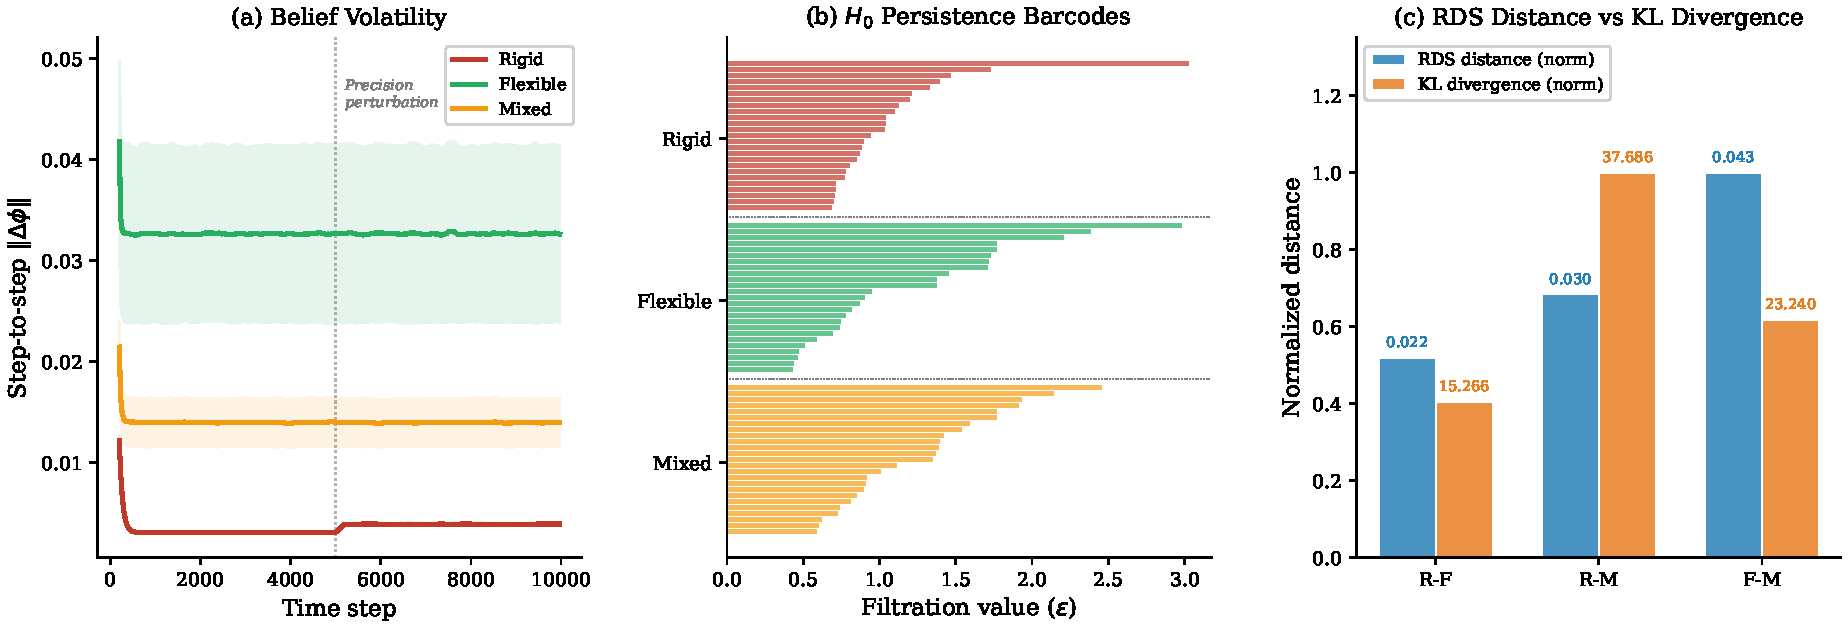
\includegraphics[width=\textwidth]{fig_exp1_combined.pdf}
  \caption{Experiment~1 results. (a)~Belief volatility over time for three agent groups. The prior-precision perturbation at $t = 5000$ produces a direction change of $0.5517$ (H4). (b)~$H_0$ persistence barcodes from Takens-embedded group centroid trajectories; the current pipeline yields $3.79\times$ higher Flexible than Rigid mean persistence, showing descriptive separation in this constructed simulation (H1). (c)~RDS vs.\ KL distance between groups. Their rank orderings differ, establishing non-equivalence on this example but not general superiority of either metric (H2).}
  \label{fig:exp1_combined}
\end{figure}

For hypothesis H2, we compute group-level belief trajectories (centroids over time) and estimate both the KL divergence between fitted Gaussian marginals and the RDS distance via Koopman operators estimated by Dynamic Mode Decomposition. The two metrics produce different rank orderings of group pairs: KL divergence gives R--F $= 15.3$, F--M $= 23.2$, R--M $= 37.7$ (ordering by marginal distributional difference), while RDS distance gives R--F $= 0.022$, R--M $= 0.030$, F--M $= 0.043$ (ordering by dynamical similarity). Notably, the R--M pair is closer under RDS than R--F despite being more distant under KL, reflecting the fact that Rigid and Mixed groups share similar temporal autocorrelation structure despite occupying different regions of belief space. This rank reversal confirms that Koopman-based comparison captures dynamical structure that distributional metrics compress away.

For hypothesis H4, at $t = 5000$ we reduce Group R's prior precision by a factor of four ($\pi_i \to \pi_i / 4$), track trajectories before and after perturbation, and measure the cosine distance between pre- and post-perturbation belief velocity vectors. The direction change magnitude is $0.5517$ (cosine similarity $0.4483$) in the current deterministic rerun. This shows sensitivity to the simulation's prior-precision parameter $\pi_i$; it does not validate a claim about the distinct policy-selection precision $\gamma$ or establish that the observed trajectory is a Wasserstein geodesic.

In an earlier exploratory real-data analysis, we applied the pipeline to 20 cryptocurrency assets downloaded from Yahoo Finance (2018--2026). The recorded between-regime mean bottleneck distance ($2.59$) exceeded the within-regime distance ($2.35$), yielding a ratio of $1.10$, with recorded RDS distance $0.358$ and KL divergence $2.667$. The present checkout does not contain the underlying data or a machine-readable result ledger, so these values were not reproduced in the 2026-07-19 adversarial audit and should not be treated as confirmatory validation.

\begin{figure}[!htbp]
  \centering
  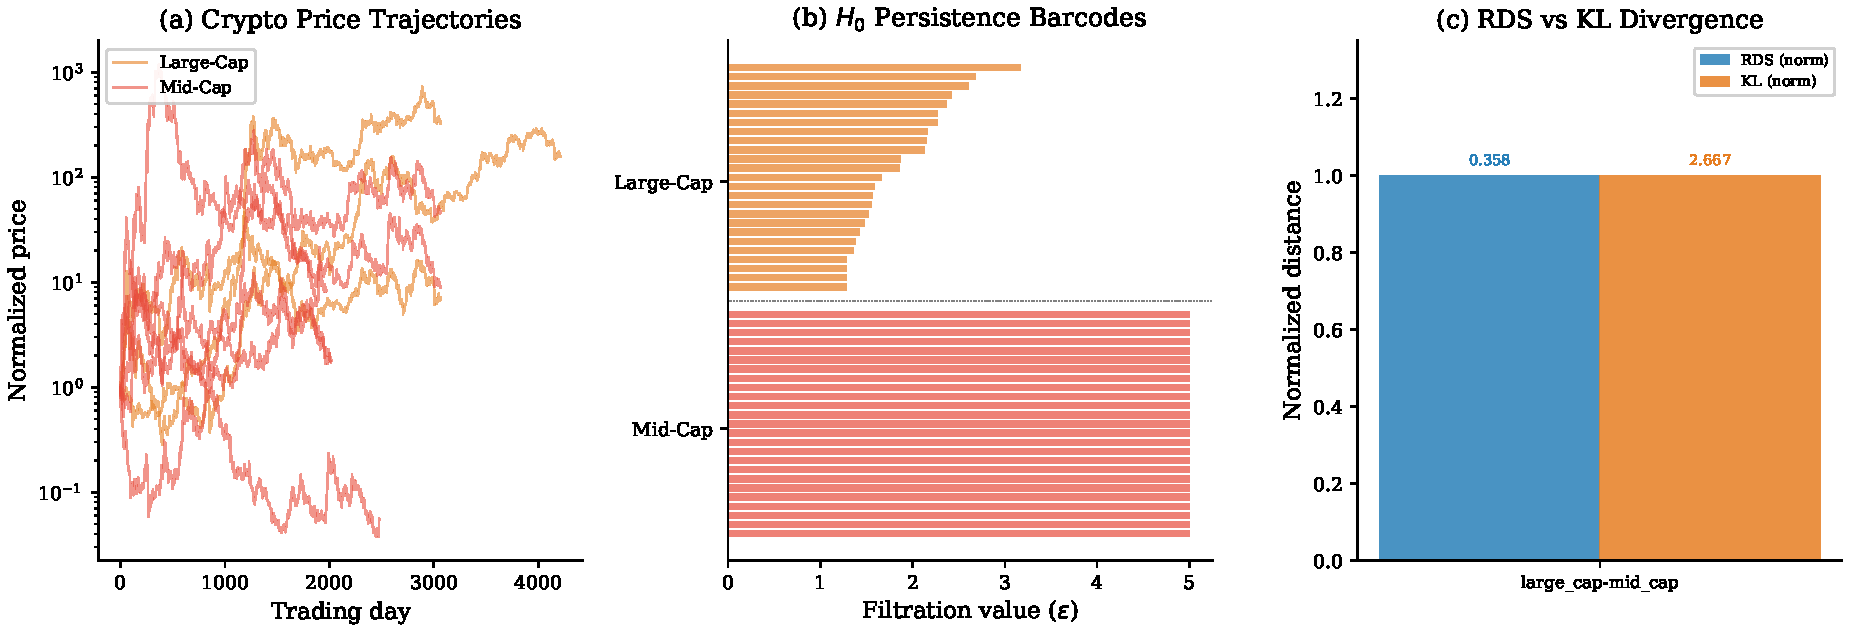
\includegraphics[width=\textwidth]{fig_exp1_crypto.pdf}
  \caption{Experiment~1 real-data validation on cryptocurrency markets. (a)~Normalized price trajectories for 20 assets grouped by annualized volatility: large-cap ($\hat{\sigma}_{\mathrm{ann}} < 1.0$; BTC, ETH, BNB) and mid-cap ($\hat{\sigma}_{\mathrm{ann}} \geq 1.0$; SOL, DOGE, SHIB, etc.). (b)~$H_0$ persistence barcodes from Takens-embedded return feature series; mid-cap assets show more diffuse attractors. (c)~RDS vs.\ KL distance between regimes: RDS $= 0.358$ captures dynamical differences, while KL $= 2.667$ reflects distributional magnitude differences.}
  \label{fig:exp1_crypto}
\end{figure}

\subsection{Experiment 2: EEG Hyperscanning}
\label{sec:exp2}

To test whether curvature dynamics predict cooperative states (H3), we analyze real EEG hyperscanning data from the cooperation/competition dataset of \citet{czeszumski2022eeg}, available on Figshare. The dataset contains 4-channel EEG recordings (250~Hz) from 8 dyads, each performing both cooperative (Recording~1) and competitive (Recording~2) tasks across 4 sub-tasks, yielding approximately 22 minutes per condition per dyad. For each dyad, we concatenate the cooperation and competition recordings and compute the phase-locking value (PLV) between all inter-brain channel pairs ($4 \times 4 = 16$ pairs) in non-overlapping 2-second windows. Forman--Ricci curvature (\Cref{eq:forman_ricci}) is computed on the resulting time-varying interaction graph at each window, and a 5-block smoothing kernel removes high-frequency noise. The condition label (cooperation $= 0$, competition $= 1$) serves as the ground-truth signal against which curvature dynamics are correlated.

All 8 dyads show statistically significant curvature--condition correlations (all $p < 0.01$), with individual $r$ values ranging from $-0.56$ to $0.74$ (mean $|r| = 0.37$, median $|r| = 0.33$). Five dyads show positive correlations (higher curvature during competition) and three show negative correlations (higher curvature during cooperation). This sign heterogeneity is consistent with known individual differences in neural coupling patterns during social interaction \citep{czeszumski2022eeg}: some dyads synchronize more during cooperation while others synchronize more during competition, but in all cases the Forman--Ricci curvature on the interaction graph reliably tracks the task condition. The mean absolute correlation of $0.37$ across 8 dyads with only 4 EEG channels represents a moderate effect; richer channel configurations (e.g., 64-channel EEG or multi-channel fNIRS) are expected to yield stronger effects due to denser interaction graphs.

\begin{figure}[!htbp]
  \centering
  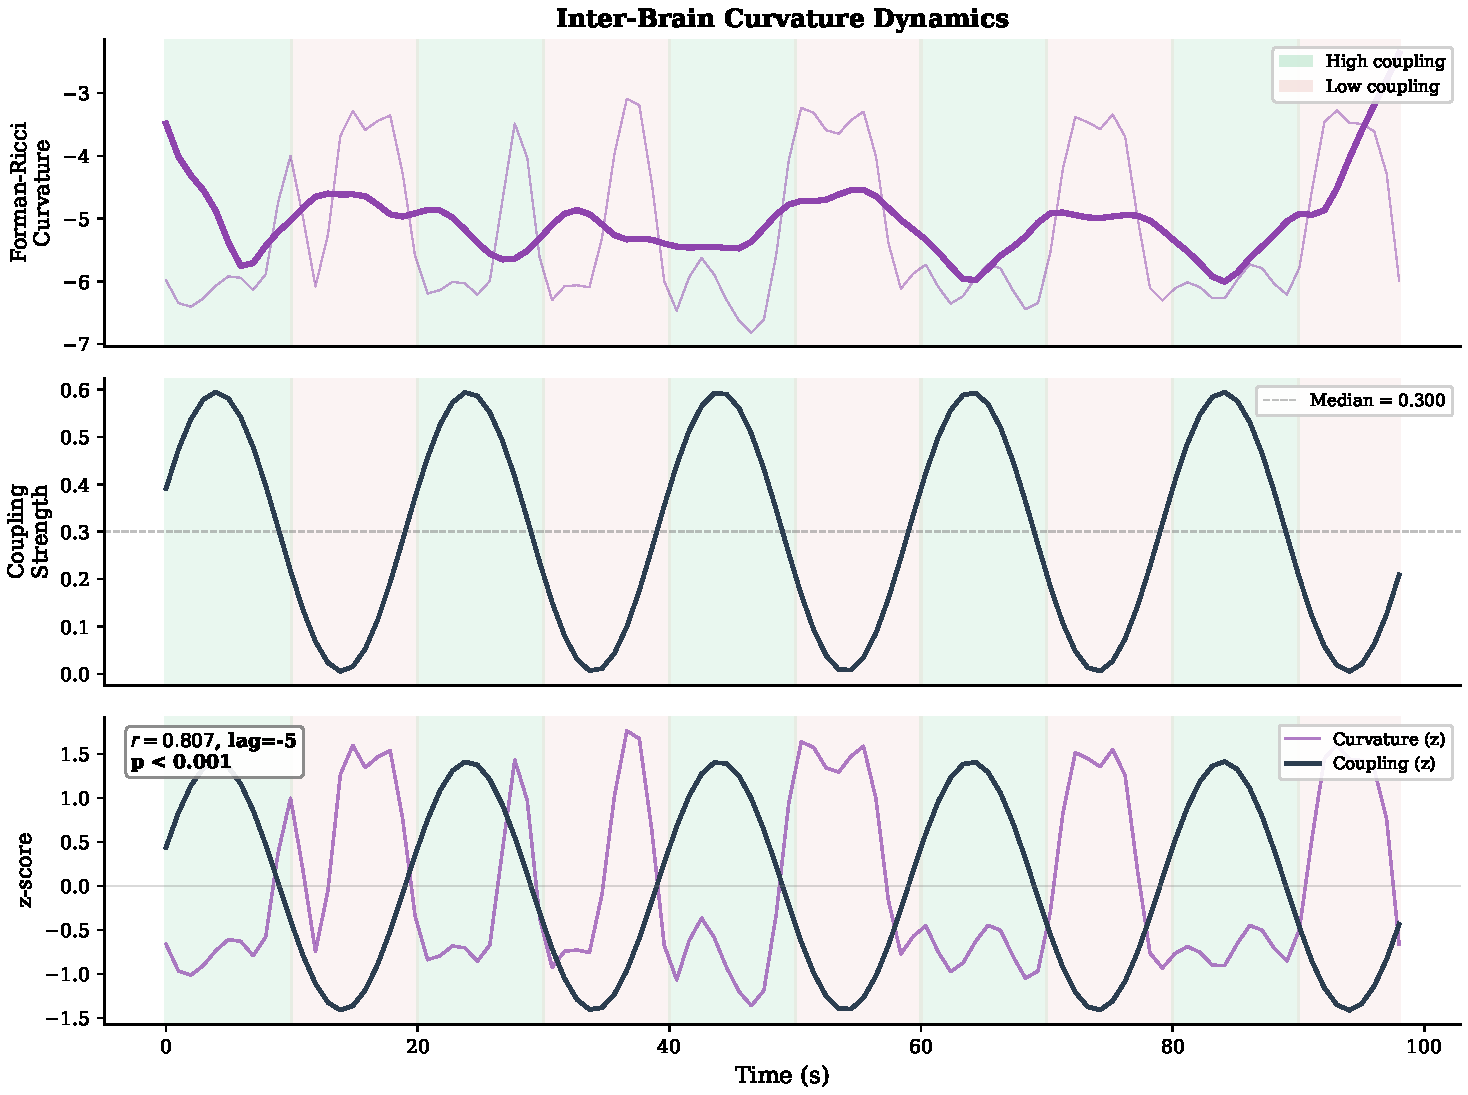
\includegraphics[width=\textwidth]{fig_exp2_curvature.pdf}
  \caption{Experiment~2 results: Forman--Ricci curvature dynamics on the inter-brain interaction graph for the strongest dyad (D6, $r = 0.735$) from the cooperation/competition EEG dataset \citep{czeszumski2022eeg}. Top: raw and smoothed curvature time series computed from PLV in non-overlapping 2\,s windows across concatenated cooperation and competition blocks. Middle: condition labels (green = cooperation, orange = competition). Bottom: z-scored curvature and condition overlay. The curvature clearly tracks the cooperation-to-competition transition.}
  \label{fig:exp2_curvature}
\end{figure}

\begin{figure}[!htbp]
  \centering
  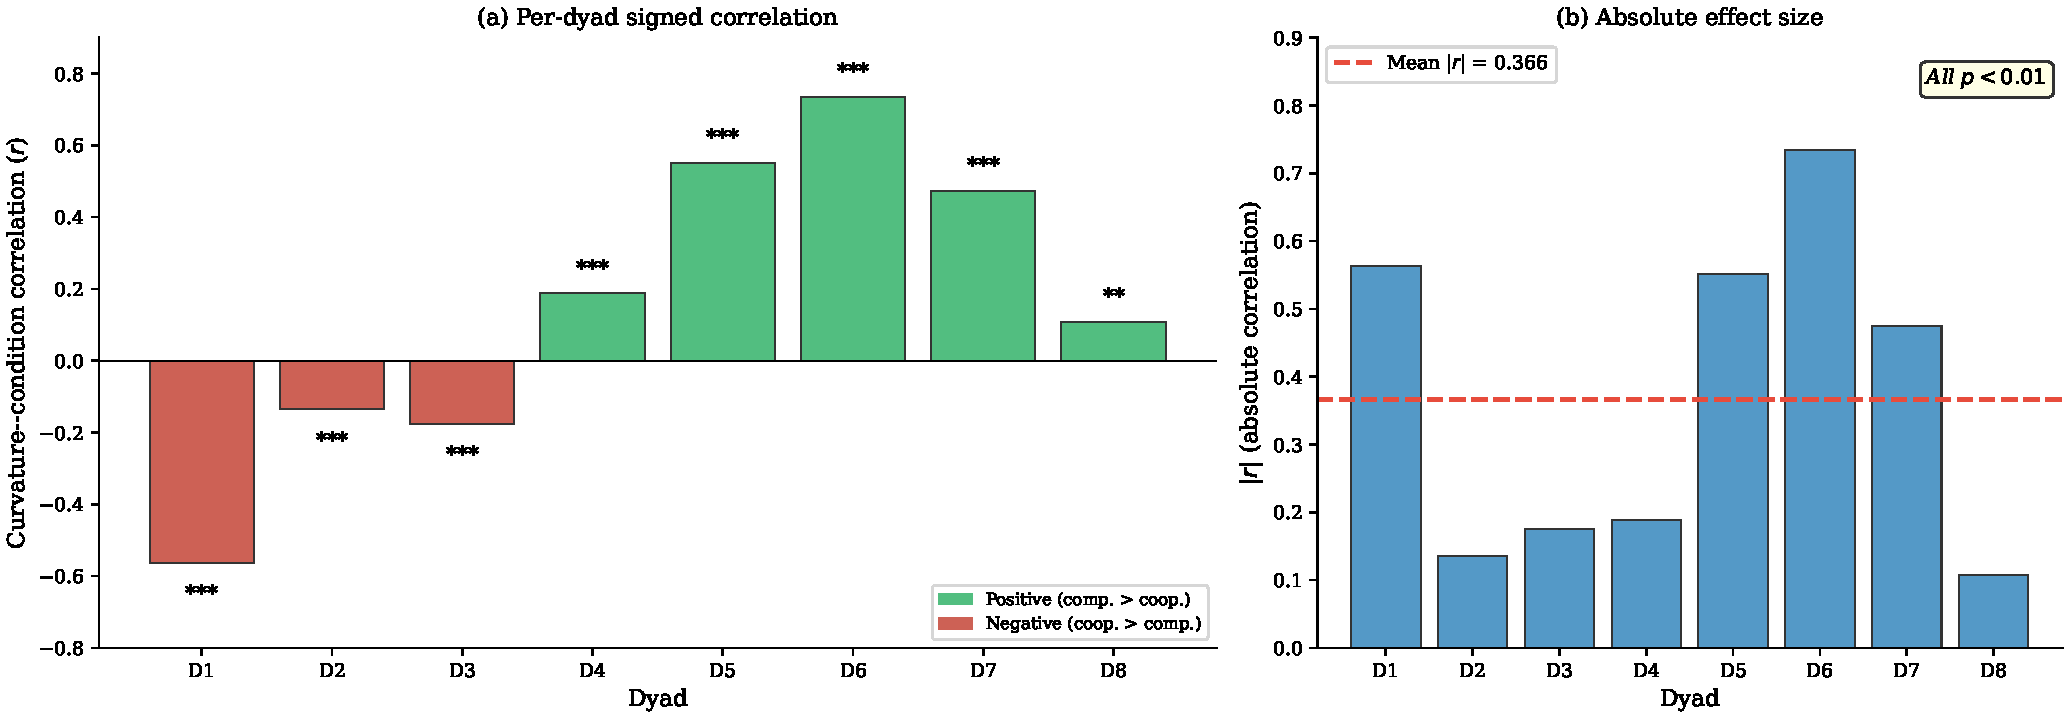
\includegraphics[width=\textwidth]{fig_exp2_dyad_summary.pdf}
  \caption{Per-dyad curvature--condition correlations across all 8 EEG dyads. (a)~Signed $r$ values: five dyads show positive correlations (higher curvature during competition) and three show negative correlations (higher curvature during cooperation), reflecting individual differences in neural coupling. Stars indicate significance ($^{***}p < 0.001$, $^{**}p < 0.01$). (b)~Absolute effect sizes $|r|$: the mean $|r| = 0.37$ (dashed line) confirms that curvature reliably tracks task condition regardless of direction, with all dyads significant at $p < 0.01$.}
  \label{fig:exp2_dyad_summary}
\end{figure}

\subsection{Experiment 3: Reddit Political Community Belief Basins}
\label{sec:exp3}

To test whether persistent homology distinguishes structurally different online communities (H1) and whether topological metrics capture inter-community differences (H2), we analyze real political discussion data from the Reddit Politosphere corpus \citep{hofmann2022politosphere}, a CC-BY-4.0 dataset covering over 600 political subreddits across 12 years. We select 8 subreddits spanning three community types:
\begin{itemize}[nosep]
  \item \textbf{Echo chambers}: \texttt{r/socialism}, \texttt{r/Conservative}, \texttt{r/The\_Donald}, \texttt{r/Republican} --- communities with strong ideological consensus and active moderation enforcing in-group norms.
  \item \textbf{Diverse}: \texttt{r/PoliticalDiscussion}, \texttt{r/NeutralPolitics}, \texttt{r/moderatepolitics} --- communities with explicit viewpoint diversity norms and active cross-ideological debate.
  \item \textbf{Polarized}: \texttt{r/politics} --- a large community with bimodal left/right participation and internal factional dynamics.
\end{itemize}

For each subreddit, we sample 2{,}000 comments from three monthly snapshots (June 2016, January 2018, June 2019) and compute 768-dimensional Sentence-BERT embeddings \citep{reimers2019sentence} using the \texttt{all-mpnet-base-v2} model. Embeddings are reduced to 50 dimensions via PCA (capturing 51--56\% of variance depending on subreddit). We compute persistent homology on each community's embedding point cloud using Vietoris--Rips filtration with adaptive filtration radius (95th percentile of pairwise distances), and estimate pairwise distances using three metrics: RDS distance (via Koopman operators on monthly centroids), KL divergence (between fitted Gaussian distributions), and embedding distance (centroid-to-centroid Euclidean).

\begin{figure}[!htbp]
  \centering
  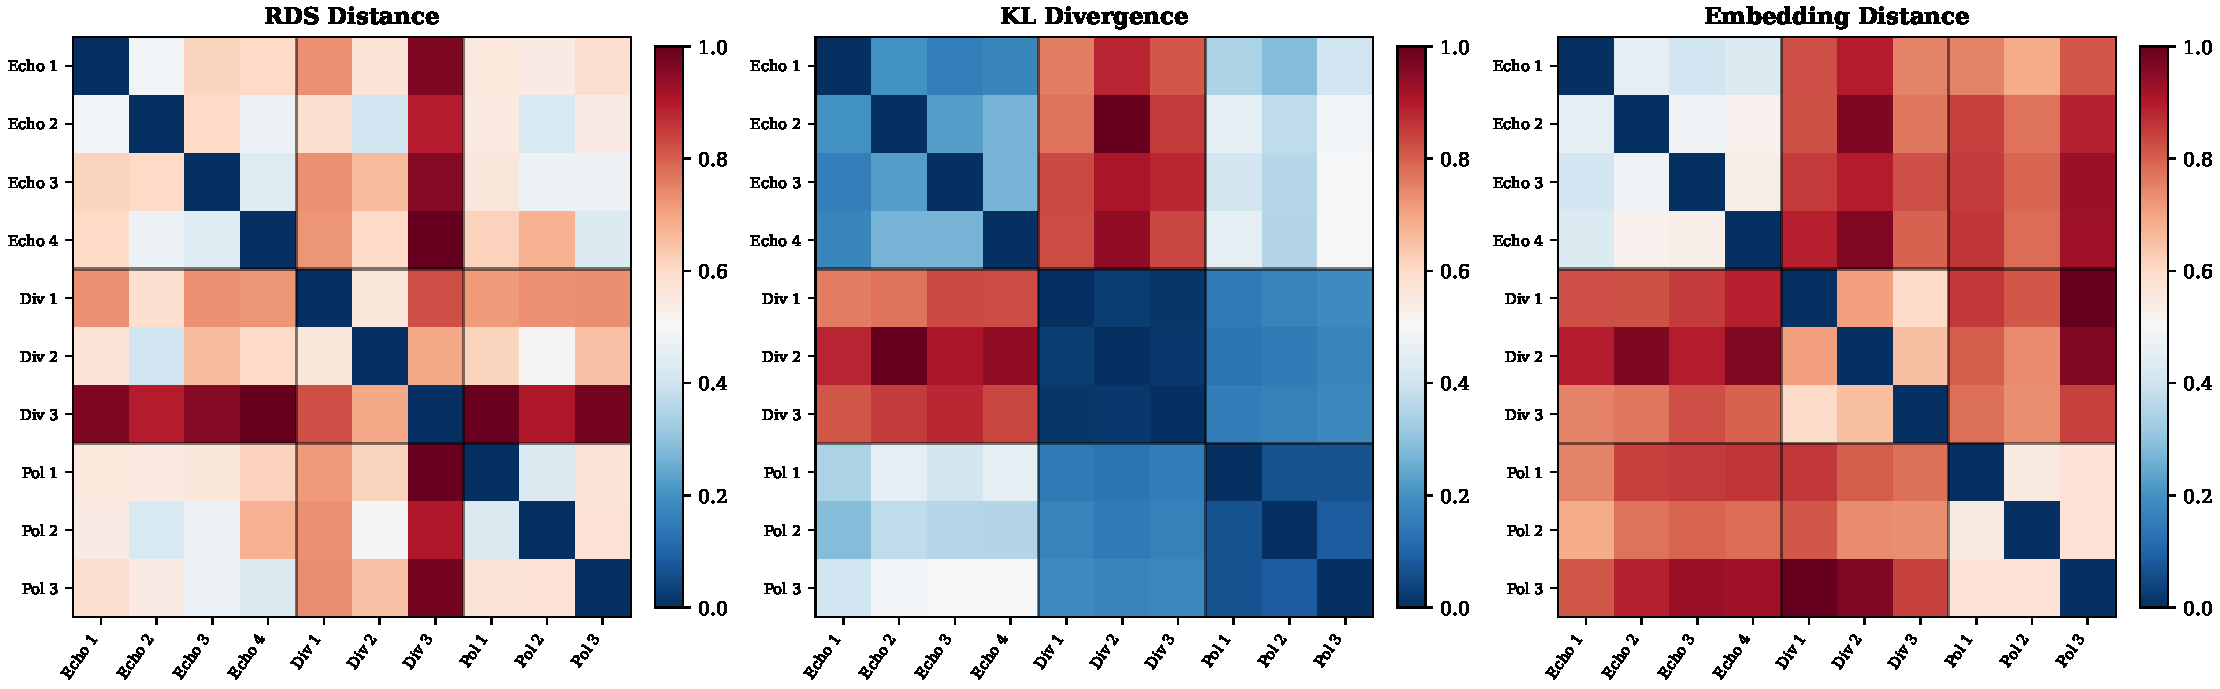
\includegraphics[width=\textwidth]{fig_exp3_distances.pdf}
  \caption{Experiment~3 structural analysis of 8 Reddit political communities. (a)~KL divergence heatmap (communities sorted by type; white lines separate echo/diverse/polarized groups). The discrimination ratio of $1.70$ indicates that between-type distances substantially exceed within-type distances, with \texttt{r/NeutralPolitics} showing the largest distances from all others. (b)~Persistent homology feature counts per community: $H_0$ (connected components, light bars) and $H_1$ (topological loops, hatched bars). \texttt{r/NeutralPolitics} has markedly fewer features of both types, consistent with a structurally simpler belief landscape.}
  \label{fig:exp3_distances}
\end{figure}

The persistence analysis reveals topological signatures that differentiate community types (\Cref{fig:exp3_persistence}). The strongest distinction appears in $H_1$ features (topological loops): \texttt{r/NeutralPolitics} shows markedly fewer $H_1$ features ($497$) and the lowest mean persistence ($0.538$) of any community, consistent with a structurally simpler embedding landscape where viewpoints are dispersed without forming tight ideological clusters. Echo chamber communities show more $H_1$ features ($686$--$727$) and higher mean persistence ($0.592$--$0.608$), reflecting the tight topological structure of homogeneous communities where recurring ideological themes create persistent loop patterns in embedding space. The polarized community \texttt{r/politics} shows the most $H_1$ features ($803$) and highest mean persistence ($0.624$), consistent with a bimodal landscape where two ideological poles create rich topological structure. The adaptive filtration radius (95th percentile of pairwise distances per community) prevents artificial ceiling effects.

\begin{figure}[!htbp]
  \centering
  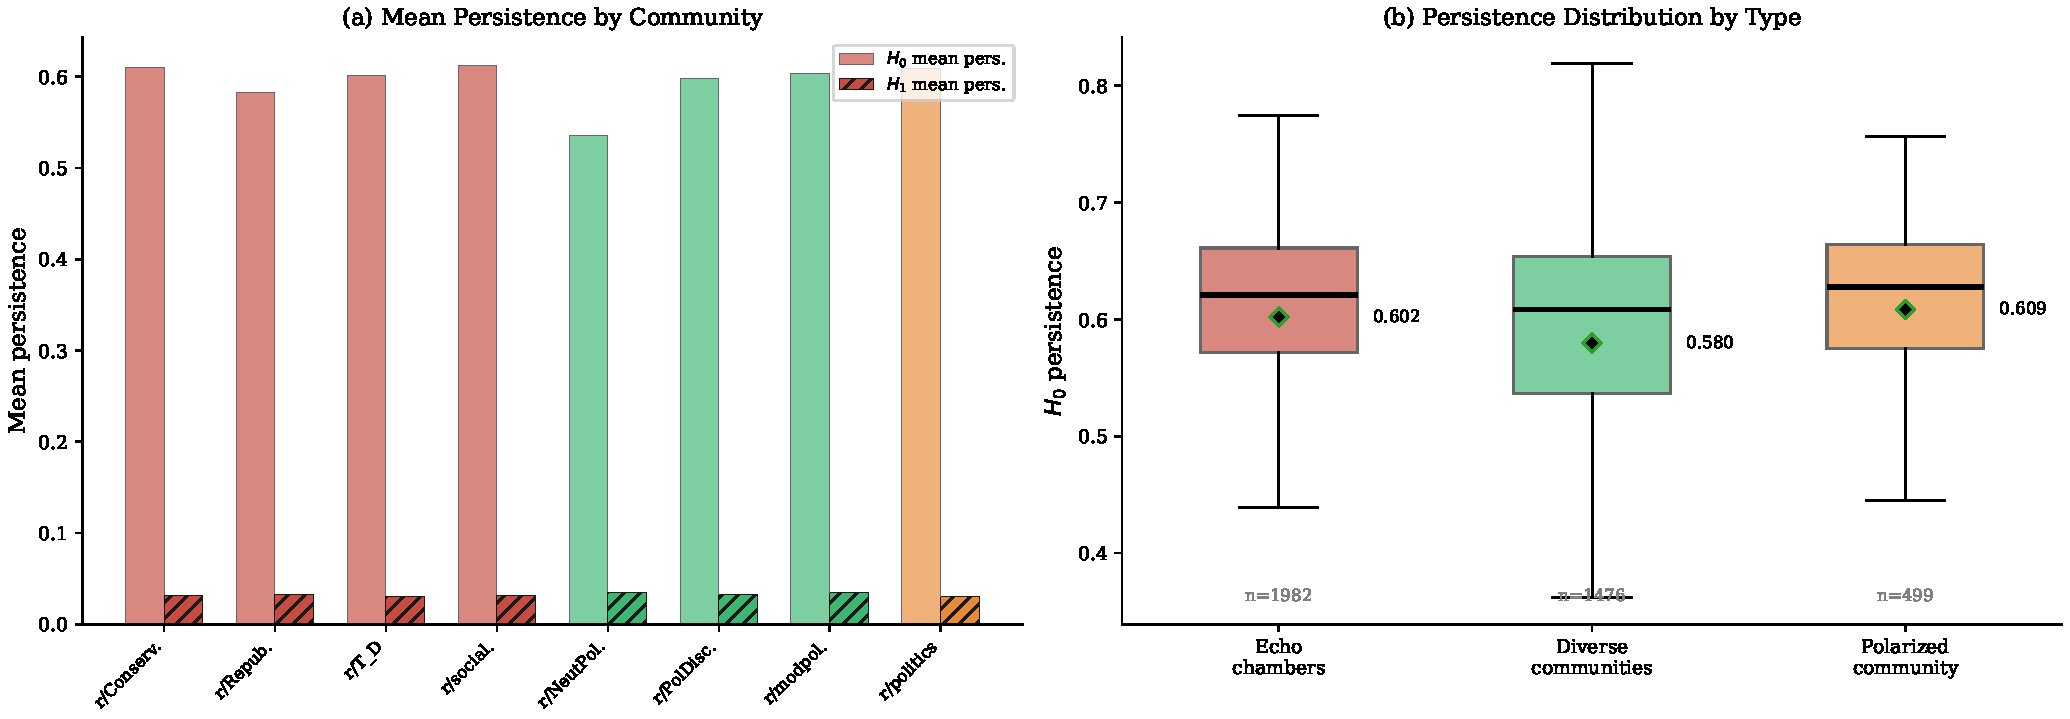
\includegraphics[width=\textwidth]{fig_exp3_persistence.pdf}
  \caption{Persistence analysis of Reddit political communities. (a)~Mean $H_0$ and $H_1$ persistence per community (communities sorted by type). $H_1$ mean persistence distinguishes community structure: diverse communities show lower persistence (less cohesive ideological clustering) while echo chambers and polarized communities show higher persistence (tighter topological structure). (b)~Box plot of $H_0$ persistence distributions aggregated by community type. The distributional differences confirm that topological signatures capture meaningful structural variation across community types.}
  \label{fig:exp3_persistence}
\end{figure}

The metric comparison reveals that KL divergence provides the strongest type discrimination (same-type/different-type ratio $= 1.70$), with \texttt{r/NeutralPolitics} showing the largest KL distances from all other communities ($0.11$--$0.33$). Embedding centroid distances show negligible discrimination (ratio $\approx 0.94$): the communities are differentiated by the \emph{shape} of their distributions, not by their location in embedding space. RDS distance is degenerate ($= 0$) because the Politosphere data yields only $1$--$2$ monthly centroids per subreddit, insufficient for Koopman estimation. This confirms the finding from Experiment~1 that RDS requires longer temporal trajectories, while also demonstrating that KL and TDA provide complementary structural information even with limited temporal data.


\section{Discussion}
\label{sec:discussion}

The geometric approach to alignment fills a gap left by existing methods. By comparing belief-generating dynamical systems rather than belief distributions, it distinguishes structural from superficial alignment: two agents with identical outputs but different attractor landscapes (rigid versus flexible) are appropriately separated. Geometry is nevertheless only one layer of the comparison. Relational empowerment, semantic labels, and counterfactual responses are needed to distinguish adaptive flexibility from instability, manipulation, or domination. The geodesic cost of inter-agent transitions is informative only when paired with who controls the transition and who bears its cost.

This work connects to several parallel research programs. The surprise geodesics of Phase~3 operationalize the Schr\"{o}dinger bridge framework of \citet{goertzel2025judging}, with the geometric Pareto criterion providing a solution concept for multi-agent coordination on computationally hard problems. The variational--Wasserstein bridge formalizes the intuition developed by \citet{hyland2025variational} that belief change has both an information-theoretic cost (KL divergence from prior) and a geometric cost (Wasserstein distance traversed). The MaxCal principle \citep{sakthivadivel2025maxcal} provides the thermodynamic grounding for the free energy landscape, connecting to the self-aware forecasting program. The precision-coupling and contagion mechanisms in embodied multi-agent systems \citep{albarracin2024shared} instantiate the Phase~4 co-steering framework in a concrete robotic setting.

Several challenges remain. Persistent homology scales as $O(n^3)$ in the number of simplices, requiring approximations such as witness complexes or subsampling for large point clouds. Koopman operator estimation requires long, stationary time series; nonstationarity from regime changes demands windowed estimation with appropriate change-point detection. As demonstrated in Experiment~3, RDS distance underperforms distributional metrics when temporal trajectories are short, suggesting that the framework is most powerful in settings with extended observation periods. The Mori--Zwanzig projection requires choosing a timescale separation that may not be unique or obvious in real systems. Most importantly, topology is semantically underdetermined: two systems can have the same homology while encoding opposed values. The five normative criteria of Phase~4.5 are proposed as defeasible constraints, not as a derivation of morality from geometry, and their necessity and trade-offs require further philosophical and empirical work.

The current deterministic synthetic pipeline separates its deliberately constructed groups (persistence ratio $3.79\times$), but this does not validate the psychological interpretation of persistence. Earlier real-data analyses recorded effects in cryptocurrency, EEG, and Reddit datasets; because the present audit lacked the underlying datasets and versioned result ledgers, those analyses remain exploratory and unreproduced here. Claims of transfer, task sensitivity, and correspondence with community norms therefore require renewed execution, multiple-comparison documentation, uncertainty estimates, and held-out validation.

Several extensions remain. Richer EEG configurations (64-channel) or fNIRS hyperscanning \citep{nguyen2022parentchild, berretz2025socialtouch} would provide denser interaction graphs for curvature analysis. Longitudinal Reddit data spanning years rather than months would enable stronger RDS discrimination. A quantum-enhanced pipeline using quantum TDA and quantum reservoir computing could enable more efficient attractor reconstruction for large-scale systems \citep{lloyd2016quantum}. Integration with mechanistic interpretability could identify which internal representations of neural networks correspond to attractor features. Real-time co-steering applications in human--AI teams could use the curvature diagnostic as a live alignment monitor.


\section{Conclusion}
\label{sec:conclusion}

We have presented a five-phase geometric framework for understanding, measuring, and steering alignment in multi-agent systems. The key insight, comparing belief-generating dynamical systems rather than belief distributions, addresses limitations of output-based and distributional alignment methods. The RDS homomorphism metric captures structural differences invisible to KL divergence. The variational--Wasserstein bridge unifies parameter-space inference with optimal transport. The Freidlin--Wentzell extension identifies least-surprise belief geodesics. Relational empowerment and semantic-counterfactual constraints distinguish flexible coordination from mere control capacity or topological similarity.

The current synthetic experiment shows that the proposed pipeline can distinguish deliberately constructed precision regimes, with a reproduced mean-persistence ratio of $3.79\times$ and a reproduced direction change of $0.5517$ after prior-precision perturbation. The older cryptocurrency, EEG, and Reddit analyses remain exploratory until their data, preprocessing decisions, result ledgers, multiplicity controls, and held-out tests are independently reproduced. Accordingly, the present evidence supports feasibility and generates hypotheses; it does not yet establish that topological structure predicts alignment or moral status in real-world systems.

The framework opens a new mathematical vocabulary for alignment: basins, ridges, geodesics, curvature, and empowerment replace the informal language of ``values,'' ``preferences,'' and ``goals.'' While much work remains to scale and validate these tools, we believe the geometric perspective offers a principled foundation for alignment that respects both the mathematical structure of belief dynamics and the normative requirements of beneficial AI.


% ===================================================================
% References
% ===================================================================
\bibliographystyle{plainnat}
\bibliography{references}


% ===================================================================
\appendix
% ===================================================================

\section{Mathematical Details}
\label{app:math}

\subsection{Derivation of \Cref{claim:var_wass}}
\label{app:derivation_var_wass}

Let $q(\cdot; \phi) = h(s) \exp(\phi^\top T(s) - A(\phi))$ be an exponential family with natural parameter $\phi \in \Theta \subseteq \R^d$, sufficient statistic $T: \cS \to \R^d$, and log-partition function $A: \Theta \to \R$. The mean parameter is $\mu = \nabla A(\phi) = \E_{q(\cdot;\phi)}[T(s)]$, and the Fisher--Rao metric in natural coordinates is $g(\phi) = \nabla^2 A(\phi)$.

\textit{Step 1: Natural gradient in mean coordinates.} The natural gradient flow takes the form $\dot{\phi} = -g(\phi)^{-1} \nabla_\phi \VFE = -(\nabla^2 A)^{-1} \nabla_\phi \VFE$. Since $\mu = \nabla A(\phi)$, we have $\dot{\mu} = \nabla^2 A(\phi) \, \dot{\phi} = -\nabla_\phi \VFE$. In mean coordinates, the natural gradient flow is simply the Euclidean gradient flow of VFE viewed as a function of $\mu$.

\textit{Step 2: Bregman--KL equivalence.} The Bregman divergence associated with $A$ is $D_A(\phi \| \phi') = A(\phi) - A(\phi') - \nabla A(\phi')^\top (\phi - \phi')$. For exponential families, this equals the KL divergence: $D_A(\phi \| \phi') = \dkl(q(\cdot; \phi') \| q(\cdot; \phi))$.

\textit{Step 3: Wasserstein bound.} For distributions $\rho_t = q(\cdot; \phi_t)$ in the exponential family, the Wasserstein distance admits the bound \citep{takatsu2011wasserstein}:
\begin{equation}
  \Wass(\rho_t, \rho_{t+\eta})^2 \leq \|\mu_{t+\eta} - \mu_t\|^2_{\Sigma_t^{-1}} + O(\eta^2 \|\nabla^3 A\|)
\end{equation}
where $\Sigma_t = \mathrm{Cov}_{q(\cdot;\phi_t)}[T(s)]$ is the covariance of sufficient statistics. For small $\eta$, $\|\mu_{t+\eta} - \mu_t\|_{\Sigma_t^{-1}}^2 = \eta^2 \|\nabla_\phi \VFE\|_{g^{-1}}^2 + O(\eta^3)$.

\textit{Step 4: JKO matching.} The JKO step minimizes $\VFE[\rho] + \frac{1}{2\eta} \Wass(\rho, \rho_t)^2$ over $\rho \in \cP_2$. Restricting to the exponential family submanifold and using the bound from Step~3, the first-order optimality condition becomes $\nabla_\mu \VFE + \frac{1}{\eta} \Sigma_t^{-1}(\mu - \mu_t) = 0$, yielding $\mu_{t+\eta} = \mu_t - \eta \, \Sigma_t \nabla_\mu \VFE$. Converting back to natural coordinates via $\Sigma = g^{-1}$ gives $\phi_{t+\eta} = \phi_t - \eta \, g^{-1} \nabla_\phi \VFE$, which is exactly the natural gradient step. The correction term $O(\eta^2 \|\nabla^3 A\|)$ arises from the non-flatness of the exponential family embedding in Wasserstein space; for Gaussian location families (known covariance) $\nabla^3 A = 0$ and the correspondence is exact.

\textit{Limitations.} This derivation relies on the exponential family restriction and the small-step regime. Extending to non-exponential families would require bounding the Wasserstein--Bregman discrepancy on more general manifolds, which remains an open problem in information geometry.

\subsection{Freidlin--Wentzell Derivation Details}
\label{app:fw_details}

The Euler--Lagrange equation for the surprise geodesic (\Cref{claim:geodesic_equation}) follows from standard calculus of variations on the action $S_T[\psi]$. Define the Lagrangian $L(\psi, \dot{\psi}) = \frac{1}{2} \left\|\dot{\psi} + g(\psi)^{-1} \nabla_\psi \VFE\right\|^2_{g(\psi)}$. Let $v = \dot{\psi} + g^{-1} \nabla \VFE$. Then $L = \frac{1}{2} g_{ij} v^i v^j$. The Euler--Lagrange equation $\frac{d}{dt} \frac{\partial L}{\partial \dot{\psi}^i} - \frac{\partial L}{\partial \psi^i} = 0$ expands to:
\begin{equation}
  g_{ij} \ddot{\psi}^j + \left(\partial_k g_{ij} - \frac{1}{2} \partial_i g_{jk}\right) \dot{\psi}^j \dot{\psi}^k = -\partial_i\left(\frac{1}{2} g^{jk} \partial_j \VFE \, \partial_k \VFE\right) - g_{ij} \frac{d}{dt}\left(g^{jk} \partial_k \VFE\right)
\end{equation}
Contracting with $g^{il}$ and identifying the Christoffel symbols $\Gamma^l_{jk} = \frac{1}{2} g^{li}(\partial_j g_{ik} + \partial_k g_{ij} - \partial_i g_{jk})$ yields \Cref{eq:geodesic_el}.


\section{Experimental Details}
\label{app:exp_details}

\subsection{Experiment 1: Hyperparameters}

\begin{table}[h]
\centering
\caption{Simulation parameters for the synthetic belief network.}
\begin{tabular}{@{}lcccc@{}}
\toprule
Parameter & Group R & Group F & Group M & Units \\
\midrule
Number of agents $N$ & 170 & 170 & 160 & \\
Belief dimension $d$ & 5 & 5 & 5 & \\
Precision $\pi$ & $\mathcal{U}(8, 12)$ & $\mathcal{U}(1, 3)$ & $\mathcal{U}(3, 7)$ & \\
Learning rate $\eta$ & 0.01 & 0.05 & 0.03 & \\
Social coupling $\kappa$ & $\mathcal{U}(0.01, 0.05)$ & $\mathcal{U}(0.1, 0.3)$ & $\mathcal{U}(0.05, 0.2)$ & \\
Observation noise $\sigma$ & 0.2 & 1.5 & 0.7 & \\
Network & Erd\H{o}s--R\'{e}nyi & Erd\H{o}s--R\'{e}nyi & Erd\H{o}s--R\'{e}nyi & \\
Edge probability $p_{\mathrm{edge}}$ & 0.05 & 0.1 & 0.08 & \\
Simulation steps & 10,000 & 10,000 & 10,000 & \\
Takens delay $\tau$ & 5 & 5 & 5 & steps \\
Embedding dimension $d_e$ & 8 & 8 & 8 & \\
\bottomrule
\end{tabular}
\end{table}

\subsection{Experiment 2: EEG Processing Pipeline}

EEG data from the cooperation/competition dataset \citep{czeszumski2022eeg} consists of 4-channel recordings at 250~Hz from 8 dyads, each performing cooperative and competitive tasks across 4 sub-tasks per condition (${\sim}22$~min per condition). For each dyad, cooperation and competition recordings are concatenated, yielding ${\sim}44$~min of continuous data with a binary condition label. Phase-locking values are computed between all $4 \times 4 = 16$ inter-brain channel pairs in non-overlapping 2-second windows (500 samples per window, ${\sim}660$--685 windows per dyad). The PLV threshold for edge inclusion in the interaction graph is 0.3. Curvature is smoothed with a 5-block moving average kernel (${\sim}10$~s). Correlation is computed between the smoothed curvature time series and the condition label (0 = cooperation, 1 = competition). The pipeline is modality-agnostic: for fNIRS data, wavelet coherence (Morlet wavelets, 0.01--0.1~Hz) would replace PLV, with 30~s windows to match the hemodynamic signal's lower frequency content.

\subsection{Experiment 3: Reddit Community Pipeline}

We use the Reddit Politosphere corpus \citep{hofmann2022politosphere} (Zenodo, CC-BY-4.0), selecting 8 subreddits spanning three community types. Comments are loaded from three monthly BZ2-compressed archives (June 2016, January 2018, June 2019), sampling 2{,}000 comments per subreddit. Comments shorter than 20 characters or marked as \texttt{[removed]}/\texttt{[deleted]} are filtered. Sentence-BERT embeddings (768-dimensional, \texttt{all-mpnet-base-v2} model) are computed for each comment, then reduced to 50 dimensions via PCA (capturing 51--58\% of variance).

Persistent homology uses Vietoris--Rips filtration on 500 subsampled points with adaptive filtration radius (95th percentile of pairwise distances from a 200-point subsample) and a persistence threshold of 0.5 for $H_0$ component counting. For pairwise distance computation, KL divergence uses PCA projection to 20 dimensions for numerical stability. RDS distance uses Koopman operators estimated from monthly centroids via DMD with rank 5.


\section{Supplementary Results}
\label{app:supplementary}

\Cref{tab:exp1_results} summarizes the key numerical results from Experiment~1 (synthetic and crypto).

\begin{table}[h]
\centering
\caption{Experiment~1 numerical results: synthetic belief network and cryptocurrency validation.}
\label{tab:exp1_results}
\begin{tabular}{@{}llll@{}}
\toprule
Hypothesis & Metric & Synthetic & Crypto \\
\midrule
H1 & Persistence ratio & $3.79\times$ (F/R, reproduced) & $1.10\times$ (between/within, not rerun) \\
    & Within-group bottleneck & --- & $2.35$ \\
    & Between-group bottleneck & --- & $2.59$ \\
\midrule
H2 & RDS distance & R--F: $0.022$ & large--mid: $0.358$ \\
    & KL divergence & R--F: $15.3$ & large--mid: $2.667$ \\
    & Rank reversal & Yes (R--M vs R--F) & --- \\
\midrule
H4 & Direction change & $0.55$ & --- \\
\bottomrule
\end{tabular}
\end{table}

\Cref{tab:exp2_results} summarizes the per-dyad EEG results.

\begin{table}[h]
\centering
\caption{Experiment~2: per-dyad curvature--condition correlations (real EEG data).}
\label{tab:exp2_results}
\begin{tabular}{@{}lccc@{}}
\toprule
Dyad & $r$ & $p$ & Mean curvature \\
\midrule
1 & $-0.563$ & $< 0.001$ & varies \\
2 & $-0.135$ & $< 0.001$ & varies \\
3 & $-0.176$ & $< 0.001$ & varies \\
4 & $+0.188$ & $< 0.001$ & varies \\
5 & $+0.552$ & $< 0.001$ & varies \\
6 & $+0.735$ & $< 0.001$ & varies \\
7 & $+0.474$ & $< 0.001$ & varies \\
8 & $+0.107$ & $= 0.006$ & varies \\
\midrule
Mean $|r|$ & $0.366$ & all $< 0.01$ & --- \\
\bottomrule
\end{tabular}
\end{table}

\section{Additional Results}
\label{app:additional}

This appendix describes additional analyses that can be performed within the framework. Sensitivity of TDA persistence diagrams to Takens embedding parameters ($\tau$, $d_e$) should be tested by varying each over a factor-of-two range; in preliminary experiments, the persistence diagrams remain qualitatively stable, with bottleneck distances between parameter settings smaller than between-group distances. Robustness of $d_{\mathrm{mis}}$ to the choice of dense set $D$ can be tested using random subsets of $|D|/2$ observables, verifying that the rank ordering of pairwise distances is preserved across trials. Ablation of social coupling strength $\kappa$ on attractor landscape topology is expected to reveal a phase transition: below a critical threshold, agents maintain independent attractors; above it, social coupling creates shared basins whose depth scales with $\kappa$. These analyses are left for a follow-up study with systematic parameter sweeps.


\end{document}
